\documentclass[conference]{IEEEtran}
\usepackage{amsmath}
\usepackage{times}
\usepackage{verbatim}
\usepackage{subfigure}
\usepackage{color}
\usepackage{graphicx}
\usepackage{multirow}
\usepackage{epstopdf}
\usepackage{threeparttable}
\usepackage{float}
\DeclareGraphicsRule{.tif}{png}{.png}{`convert #1 `basename #1 .tif`.png}

\newcommand{\reminder}[1]{\textbf{\color{red}[** #1 **]}}  % to fix
\newcommand{\hide}[1]{} %hide
\newcommand{\vpara}[1]{\vspace{0.1in}\noindent\textbf{#1 }}
\newcommand{\para}[1]{\vspace{0.01in}\noindent\textbf{#1 }}
\newcommand{\secref}[1]{Section~\ref{#1}} %section reference
\newcommand{\Real}{\ensuremath{\mathbb{R}}}  % Real numbers
\newcommand{\figref}[1]{Figure~\ref{#1}} %section reference
\newcommand{\beq}[1]{\vspace{-0.02in}\begin{equation}#1\end{equation}\vspace{-0.02in}}
\newcommand{\beqn}[1]{\vspace{-0.03in}\begin{eqnarray}#1\end{eqnarray}\vspace{-0.03in}}
\newcommand{\beal}[1]{\vspace{-0.03in}\begin{align}#1\end{align}\vspace{-0.03in}}
\newcommand{\besp}[1]{\begin{split}#1\end{split}}
% added by Sida Gao for tables
\newcommand{\tabincell}[2]{\begin{tabular}{@{}#1@{}}#2\end{tabular}}
\hyphenation{op-tical net-works semi-conduc-tor}

\usepackage{xeCJK}
\setCJKmainfont{HiraginoSansGB-W3}
\setCJKsansfont{HiraginoSansGB-W6}
\renewcommand\baselinestretch{1.2}

\begin{document}

\title{通过时间、地点信息预测三藩市犯罪类型}


% author names and affiliations
% use a multiple column layout for up to three different
% affiliations
\author{\IEEEauthorblockN{高思达}
\IEEEauthorblockA{计35班\\
2013011413\\
gsd13@mails.tsinghua.edu.cn}
\and
\IEEEauthorblockN{魏鑫鼎}
\IEEEauthorblockA{计32班\\
2013011316\\
weixinding@gmail.com
}
\and
\IEEEauthorblockN{张浩天}
\IEEEauthorblockA{计35班\\
2013011416\\
zhang-ht13@mails.tsinghua.edu.cn
}}

\maketitle

\begin{abstract}

\reminder{
    成文后需要修改!
}

这篇文章是清华大学2016年数据挖掘课程的大作业报告。
我们小组选择参加Kaggle竞赛:三藩市犯罪分类(San Francisco Crime Classification)作为本次大作业的项目。
在该项目中,我们通过学习部分标记了犯罪类型的时间、地点数据,对另一部分未标记的时间、地点数据预测犯罪类型。
我们利用已有的数据构造了一些更高层次的特征,并使用多种模型进行预测和评价。
我们发现,我们构造的特征几乎都出现了对于训练集数据过拟合的问题,导致对于测试集的预测产生了严重的负面效果。
最终,预测效果最好的方法为,使用原始特征训练Xgboost模型进行预测,该结果在排行榜上的排名为81名(共2335支队伍,约前4\%)。

\end{abstract}
\section{引言}
\label{sec:intro}

三藩市(San Francisco)是一座在美国加州的淘金热潮中繁荣起来的城市。然而在城市快速扩张、人口迅速增加的同时,红灯区等诸多社会问题逐渐涌现出来,这些问题直接表现为犯罪率的上升。时至今日,三藩市早已不再是当年的矿镇,而已经成为了世界的一大科技中心。但是,常年高企的犯罪率却仍然没有好转。

作为科技重镇,三藩市公开了2003年至2015年的犯罪记录供数据科学家研究之用。通过挖掘这些数据,可以使得警察局能够更好地了解不同类型犯罪的趋势。通过根据时间和地点信息预测犯罪类型,警察局能够提前了解犯罪可能性更高的地区和时段,并针对性地采取措施以降低犯罪率。这个犯罪记录数据集在公开后,也成为了Kaggle网站的一个比赛。

\reminder{
    本篇文章中,第\ref{sec:problem}节对问题和数据集进行描述;
    第\ref{sec:observation}节对数据进行可视化探索分析;
    第\ref{sec:feature}节介绍特征的提取方法;
    第\ref{sec:model}节介绍使用的分类模型,并比较实验结果;
    最后,第\ref{sec:conclusion}节进行总结。
}
\section{问题描述}
\label{sec:problem}

\subsection{数据集}

本次Kaggle比赛使用的数据集来自三藩市警察局的犯罪事件数据库,包括了2003年1月1日至2015年5月13日的878049条犯罪记录(共4510天,每天平均发生约195起犯罪)。训练集和测试集使用隔周的方式划分,即从第一周开始,奇数周作为训练集,偶数周作为测试集。

在数据中,犯罪细节描述(Description)和犯罪解决方式(Resolution)两个字段只有训练集才有,因此我们无法利用这些信息。
除此之外,我们可以利用的字段如下:

\begin{itemize}
    \item \textbf{Date:}犯罪案件的时间戳,包括年、月、日、时、分、秒。
    \item \textbf{DayofWeek:}
    犯罪案件发生在星期几。
    \item \textbf{PdDistrict:}
    犯罪案件发生在哪个警局的管辖地区。
    \item \textbf{Address:}
    犯罪案件发生的街道地址。
    \item \textbf{X:}
    犯罪案件发生地点的经度。
    \item \textbf{Y:}
    犯罪案件发生地点的纬度。
\end{itemize}

\subsection{预测和评价}

在训练集中,额外给出了一个字段:

\begin{itemize}
    \item \textbf{Category:}犯罪类型。
\end{itemize}

该字段是预测的目标。数据集中,一共有39种犯罪类型。
在测试集上的预测结果并不是直接给出某一种确定的犯罪类型,而是需要给出该事件、地点39种犯罪类型的概率分布。竞赛进行评测的方法是,计算多分类的对数损失(multi-class logarithmic loss),即

\begin{equation*}
    logloss=\frac{1}{N} \sum_{i=1}^N \sum_{j=1}^M y_{ij} log(p_{ij})
\end{equation*}

其中,$N$是测试集样本总数;$M$是类型总数(本问题中$M=39$);$y_{ij}$为一个标志量,当样本$i$属于类型$j$时为1,否则为0;$p_{ij}$是模型对样本$i$属于类型$j$预测的概率。可见,当预测完全准确,即$p_{ij}=1$时,对损失的贡献为0;预测概率$p_{ij}$越小,对损失的贡献越大。因此,这是一个合理的对于多分类问题的评价标准。

在实验过程中,由于比赛每天限制5次提交,因此我们需要在训练集通过交叉验证来评价预测方法(特征和模型)。在交叉验证中,我们同样使用$logloss$来评价结果。
实验中,我们直接调用了Python的sklearn包中的实现。


\section{数据观察}
\label{sec:observation}

由于我们参加比赛的时候,比赛已经进行了大约8个月,Kaggle上已经有了较多公开的脚本。在这一节的分析中,一些可视化结果是参考了公开发布的脚本做出来的。值得说明的是,除了本节之外,第\ref{sec:feature}节中提到的所有数据处理和第\ref{sec:model}节中使用的模型都是我们独立实现的脚本,没有参考其他任何来源的资料。

\subsection{犯罪总量分析}

在这一小节,我们对数据集进行粗粒度的分析。即,只变化数据点的某一个字段,而对其他字段的全体可能取值统计总数,观察每个字段的取值对于犯罪总体情况的影响。所谓犯罪总体情况,就是忽略犯罪类型,关注犯罪案件的总数。这部分分析看似并不能帮助我们进行分类,但是可以先帮我们从一个比较宏观的角度看时间和地点是如何影响犯罪的。站在实际应用角度,从时间、地点等侧面统计总体犯罪情况,可以作为当地警察局部署警力的有益参考。

\begin{figure}[tb]
    \centering
    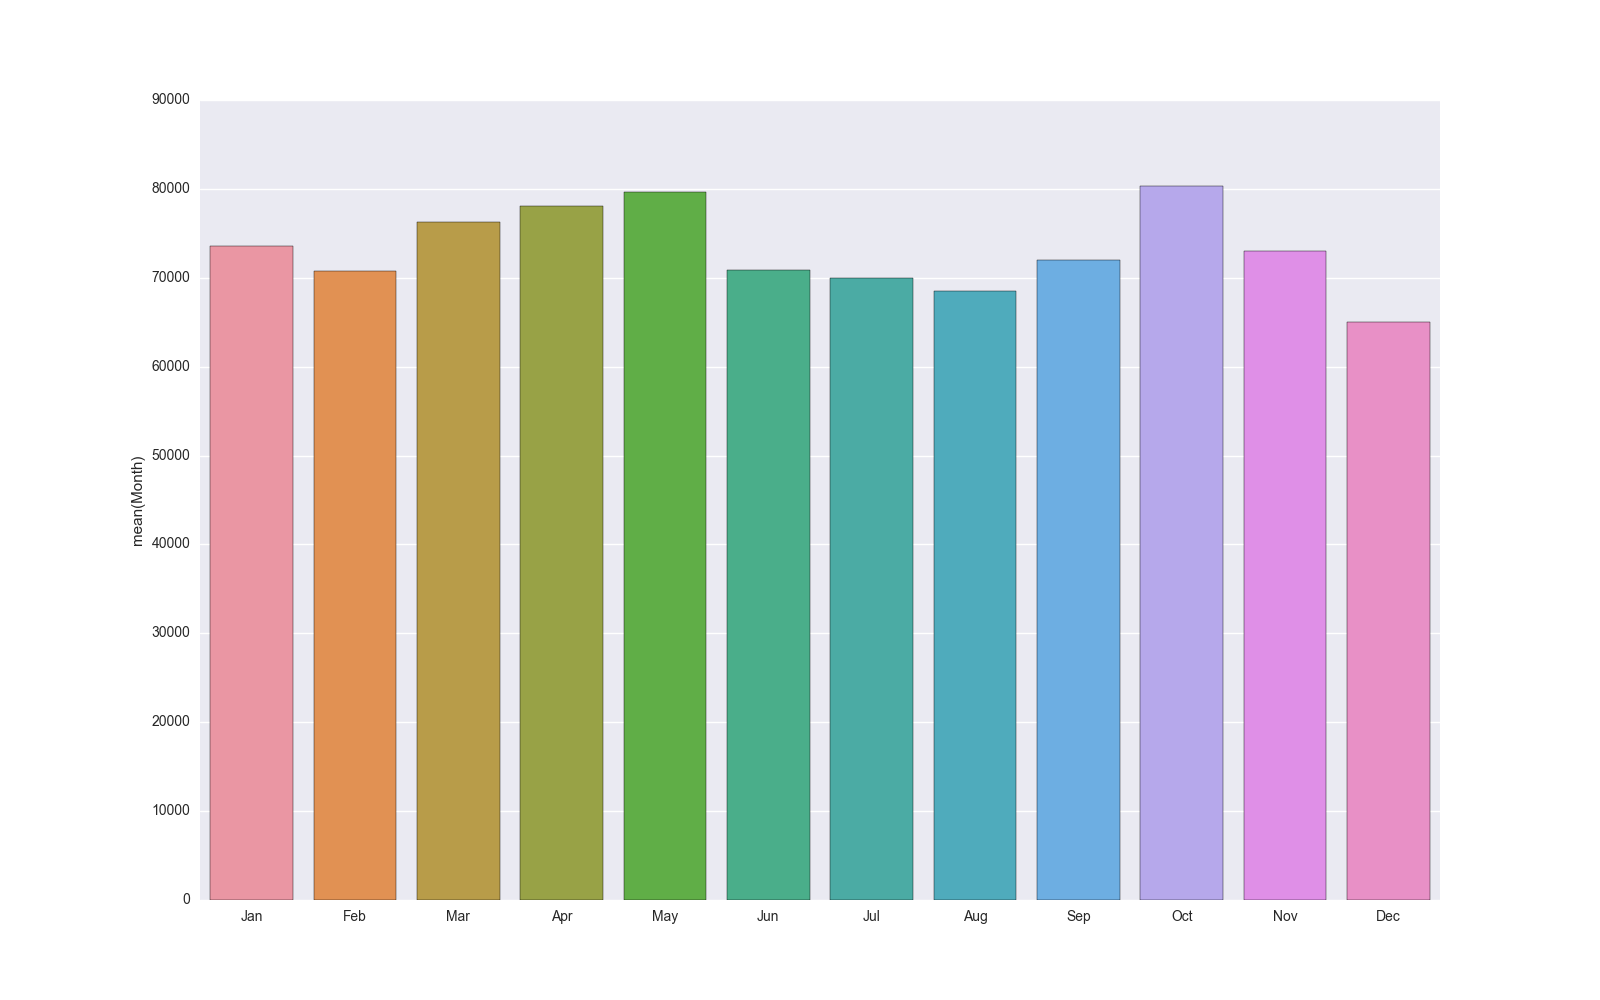
\includegraphics[width=1.0\linewidth]{fig/monthly}
    \caption{月份对犯罪总量的影响}
    \label{fig:monthly}
\end{figure}

\begin{figure}[tb]
    \centering
    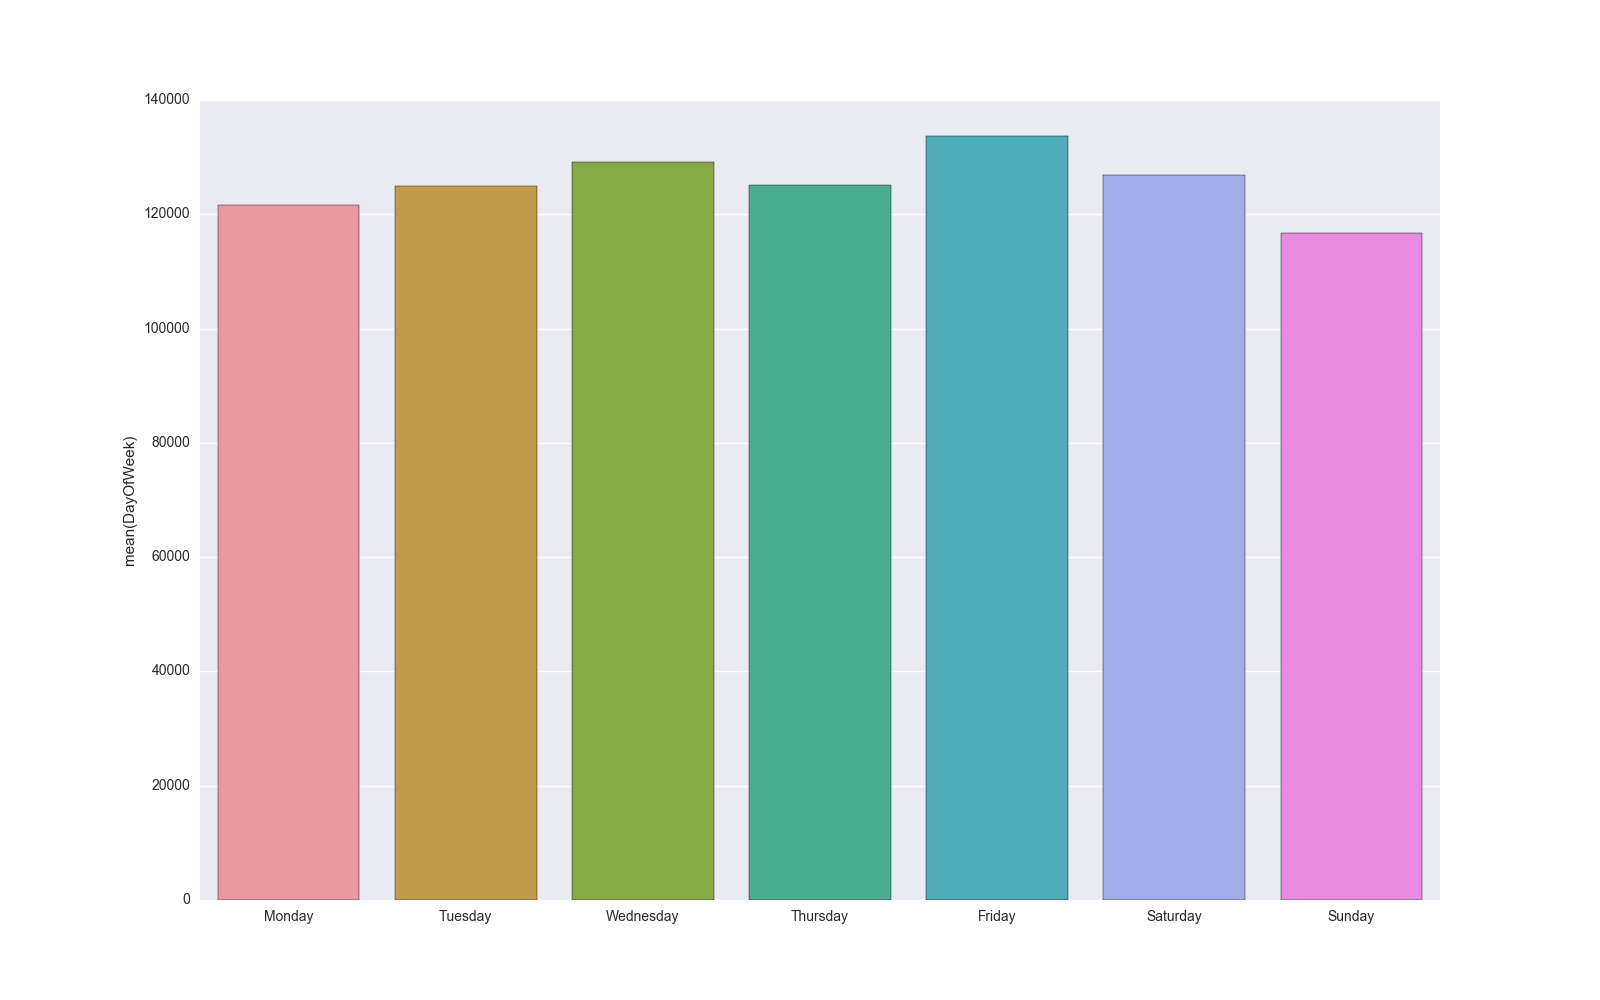
\includegraphics[width=1.0\linewidth]{fig/DayOfWeek}
    \caption{星期对犯罪总量的影响}
    \label{fig:dayofweek}
\end{figure}

\begin{figure}[tb]
    \centering
    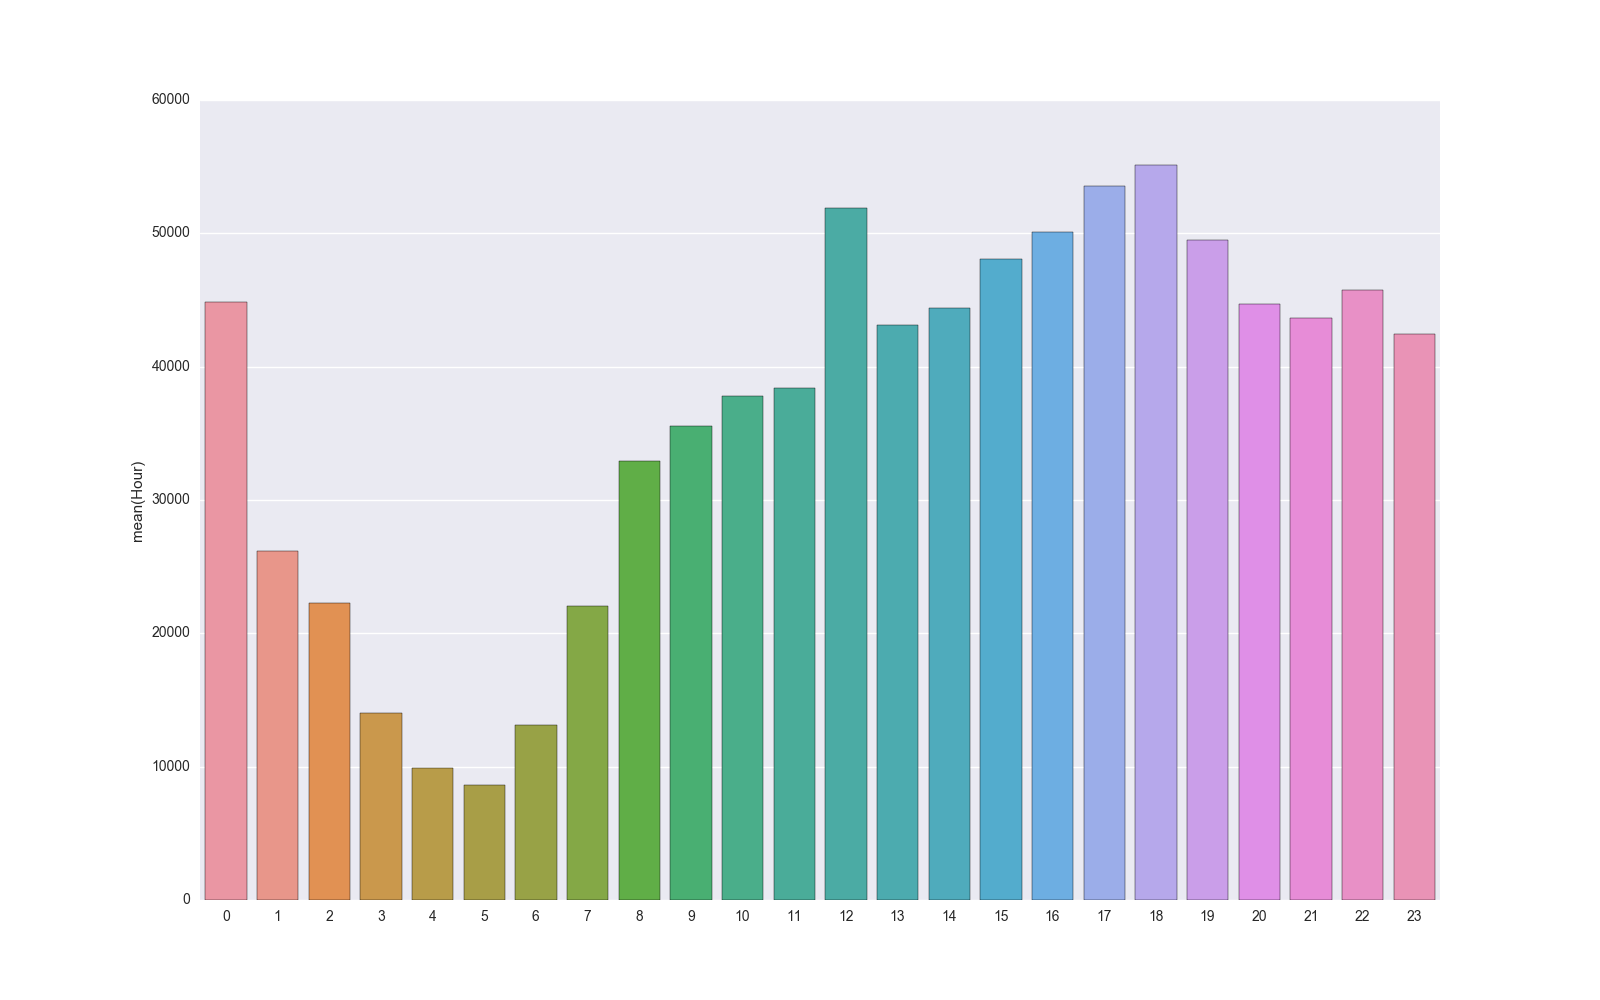
\includegraphics[width=1.0\linewidth]{fig/Hourly}
    \caption{小时对犯罪总量的影响}
    \label{fig:hourly}
\end{figure}

图\ref{fig:monthly}、图\ref{fig:dayofweek}和图\ref{fig:hourly}分别展示了月份、星期和小时对犯罪总量的影响。可见,月份变化时,犯罪总量会发生比较明显的起伏波动,但相比之下,每周的每一天的犯罪总量的变化则不那么明显。符合预期的是,小时对于犯罪的影响是最显著的:中午、傍晚和午夜有三个比较明显的犯罪高峰,而凌晨的犯罪则比较少,这一分布情况用生活经验很容易理解。

\begin{figure}[tb]
    \centering
    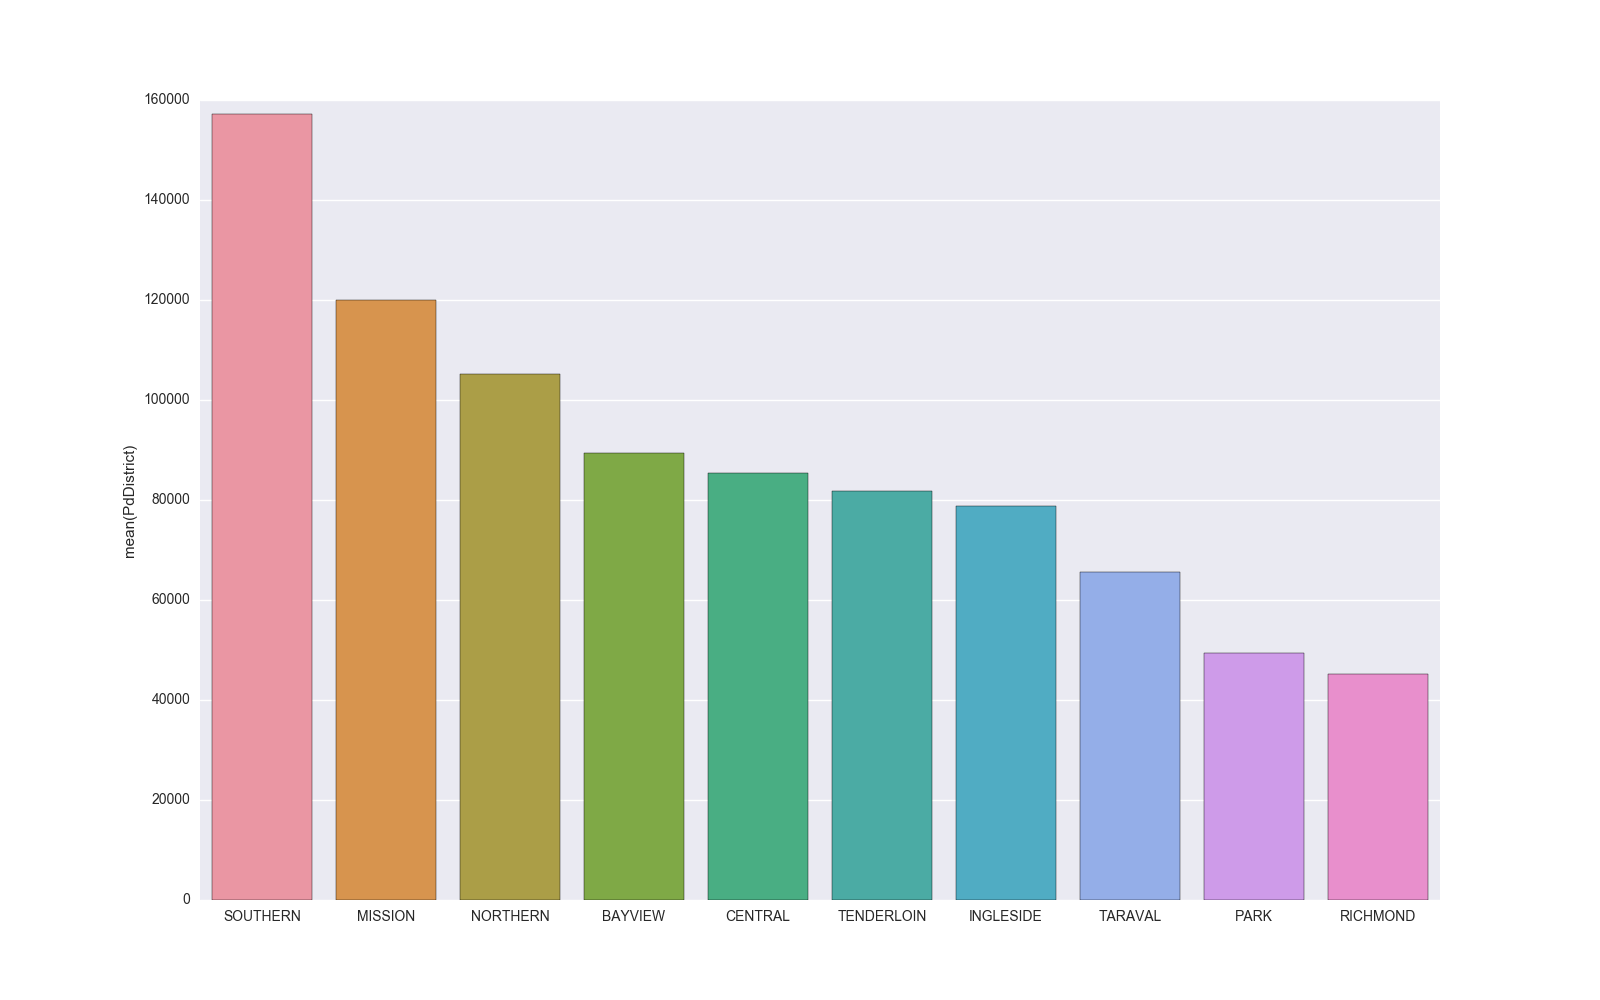
\includegraphics[width=1.0\linewidth]{fig/PdDistrict}
    \caption{各警察局片区的犯罪总量影响}
    \label{fig:pd_district}
\end{figure}

\begin{figure}[tb]
    \centering
    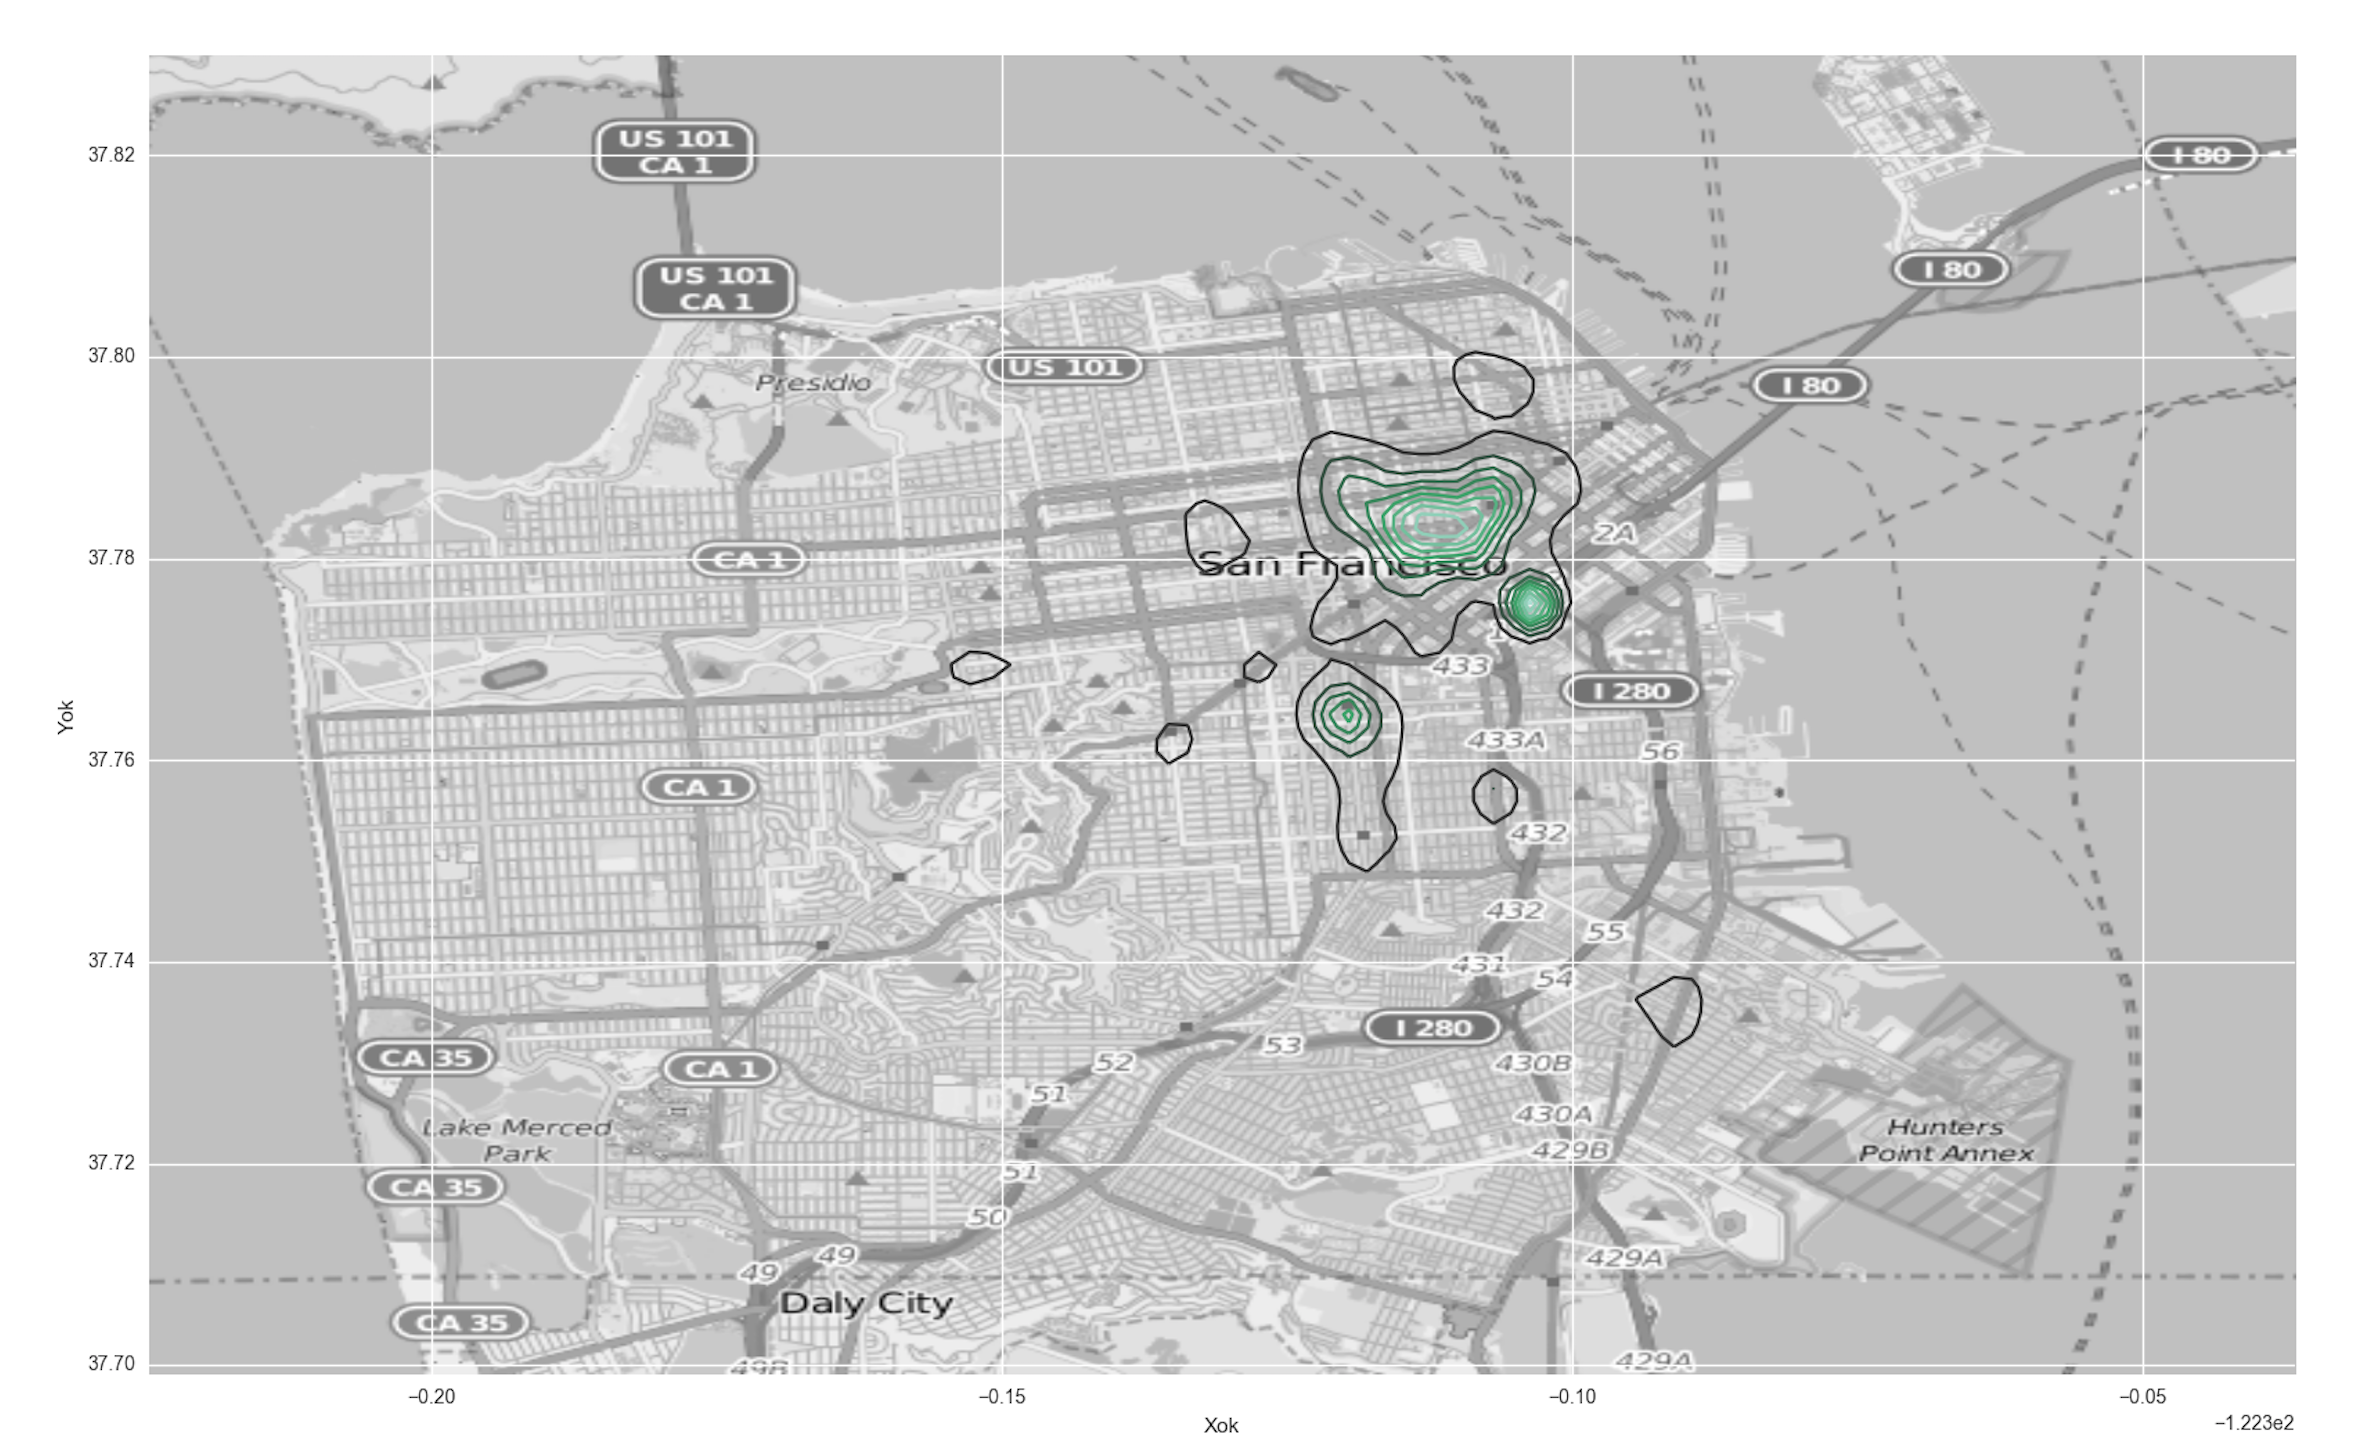
\includegraphics[width=1.0\linewidth]{fig/total_density}
    \caption{犯罪总量的热度图}
    \label{fig:tot_density}
\end{figure}

下面观察不同地点对犯罪总量的影响。首先,由图\ref{fig:pd_district}可以看出,不同警察局区域的犯罪量的差异是巨大的。由此可以推断出城市不同区域的犯罪率有巨大的不同。作为验证,我们参考Kaggle上公开的一份代码\footnote{https://www.kaggle.com/codechamp/sf-crime/crime-density-by-location/code,作者codechamp},对全部类型的犯罪总量做密度图,即图\ref{fig:tot_density}。从中可以看出,城市东北角的犯罪率要显著高于其他部分。

\subsection{犯罪类型分布的分析}

\begin{figure}[tb]
    \centering
    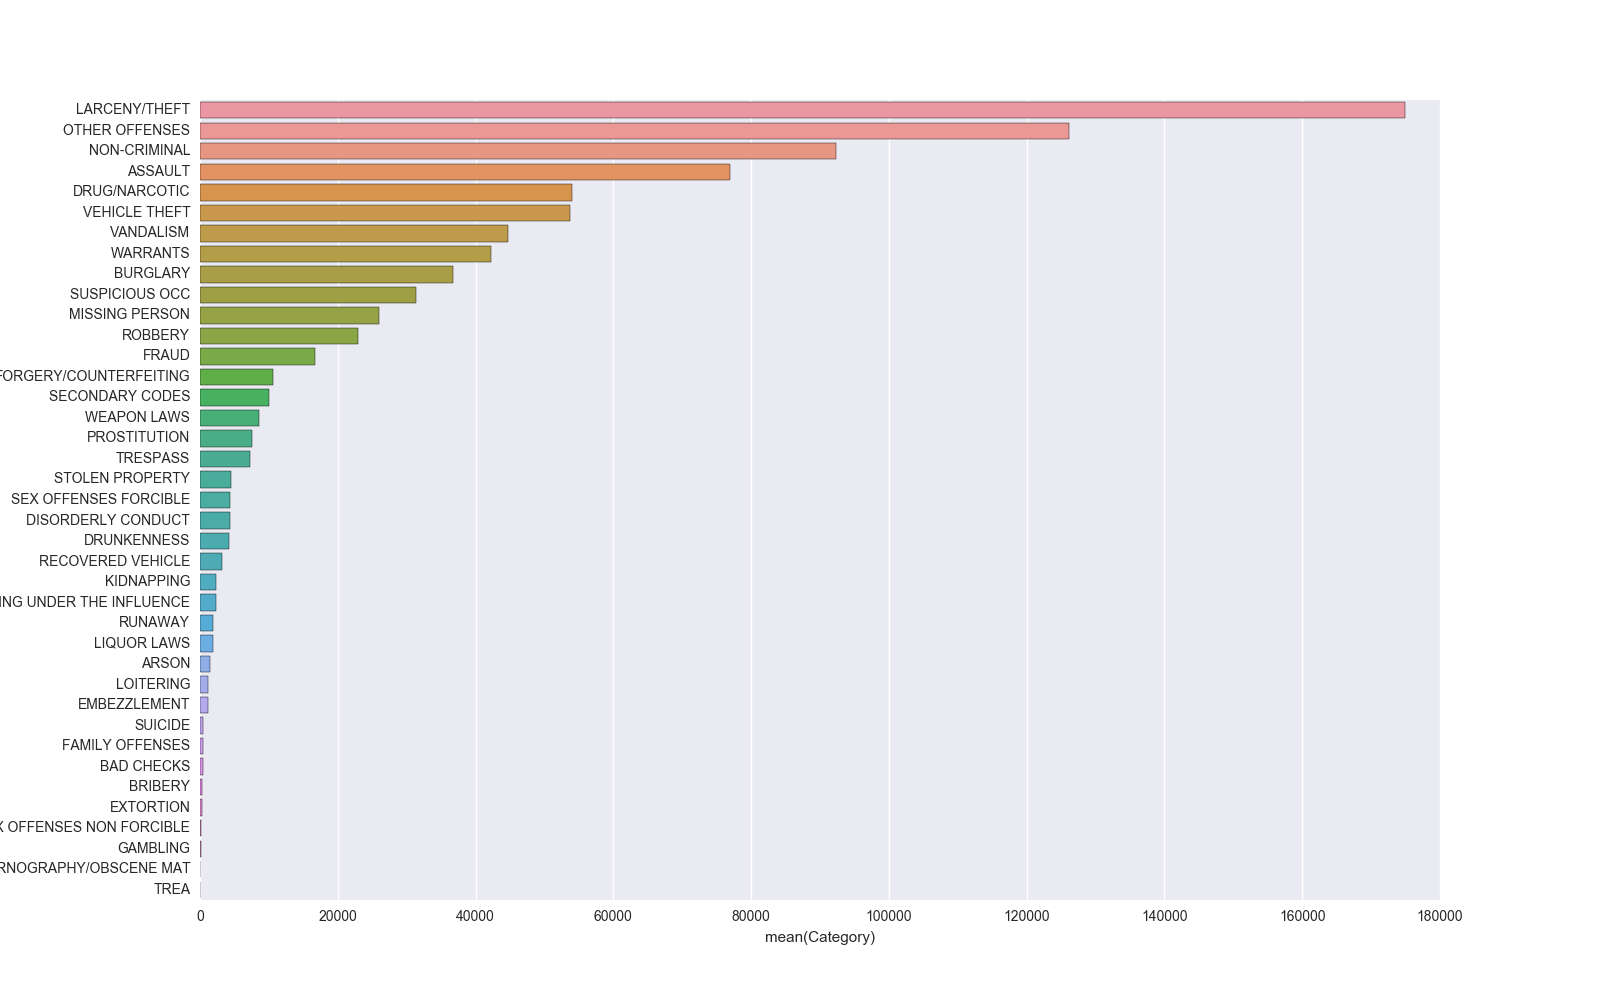
\includegraphics[width=1.0\linewidth]{fig/category}
    \caption{不同犯罪类型的总量}
    \label{fig:tot_category}
\end{figure}

首先,我们先不区分时间和地点,考察总体上各种犯罪类型的分布。图\ref{fig:tot_category}中可见,不同类型的犯罪总量是一个长尾分布,即频数最高的几个犯罪类型的总量占到了总体犯罪总数的大部分(最多的5种犯罪占整体犯罪总数的66\%)。由此可以推知,有些犯罪类型的概率总是很高的,即便一些长尾类型在某个地点集中,它的概率可能仍然没有常见类型的概率大。这种情形将会对我们的预测带来一些困难。下面,带着对犯罪类型分布的总体认识,我们进一步从地点、时间角度进行一些分析,并进一步对时间做出限制进行细粒度分析。

\subsubsection{不同犯罪类型对地点的分布}

图\ref{fig:tot_density}中已经看到了犯罪总量对于地点的分布,发现犯罪整体上趋向于同一个中心。如果每一种犯罪类型单独分析时,都趋向于这个中心,那么可以认为地点对于每种犯罪类型的概率的影响是一致的,即地点信息对于预测犯罪类型没有任何帮助。但是,图\ref{fig:tot_category}中的结果可以看到,虽然绝大多数犯罪类型都会有城市东北角的密度中心,很多犯罪类型也会有其他的密度中心。比如,纵火(ARSON)和赌博(GAMBLING)都在城市的东南角有一个密度中心。更有趣的是一个例子是,离家出走(RUNAWAY)的密度中心和其他任何一种犯罪类型的都十分不同,这应该是源于“离家出走”其实并不是真正的犯罪。总之,根据图\ref{fig:tot_category},不同犯罪类型在地点上的分布是有所不同的,所以地点信息对预测很有帮助。另外值得注意的是,频率最高的几种犯罪类型:盗窃(THEFT)、其他侵犯(OTHER OFFENSES)、无罪(NON-CRIMINAL)、攻击(ASSAULT)、吸毒(DRUG)的密度中心都集中在城市东北角,即全部犯罪类型的集中位置。也就是说,对于高频犯罪,地点信息的辨别能力不强。

\begin{figure*}[!bt]
    \centering
    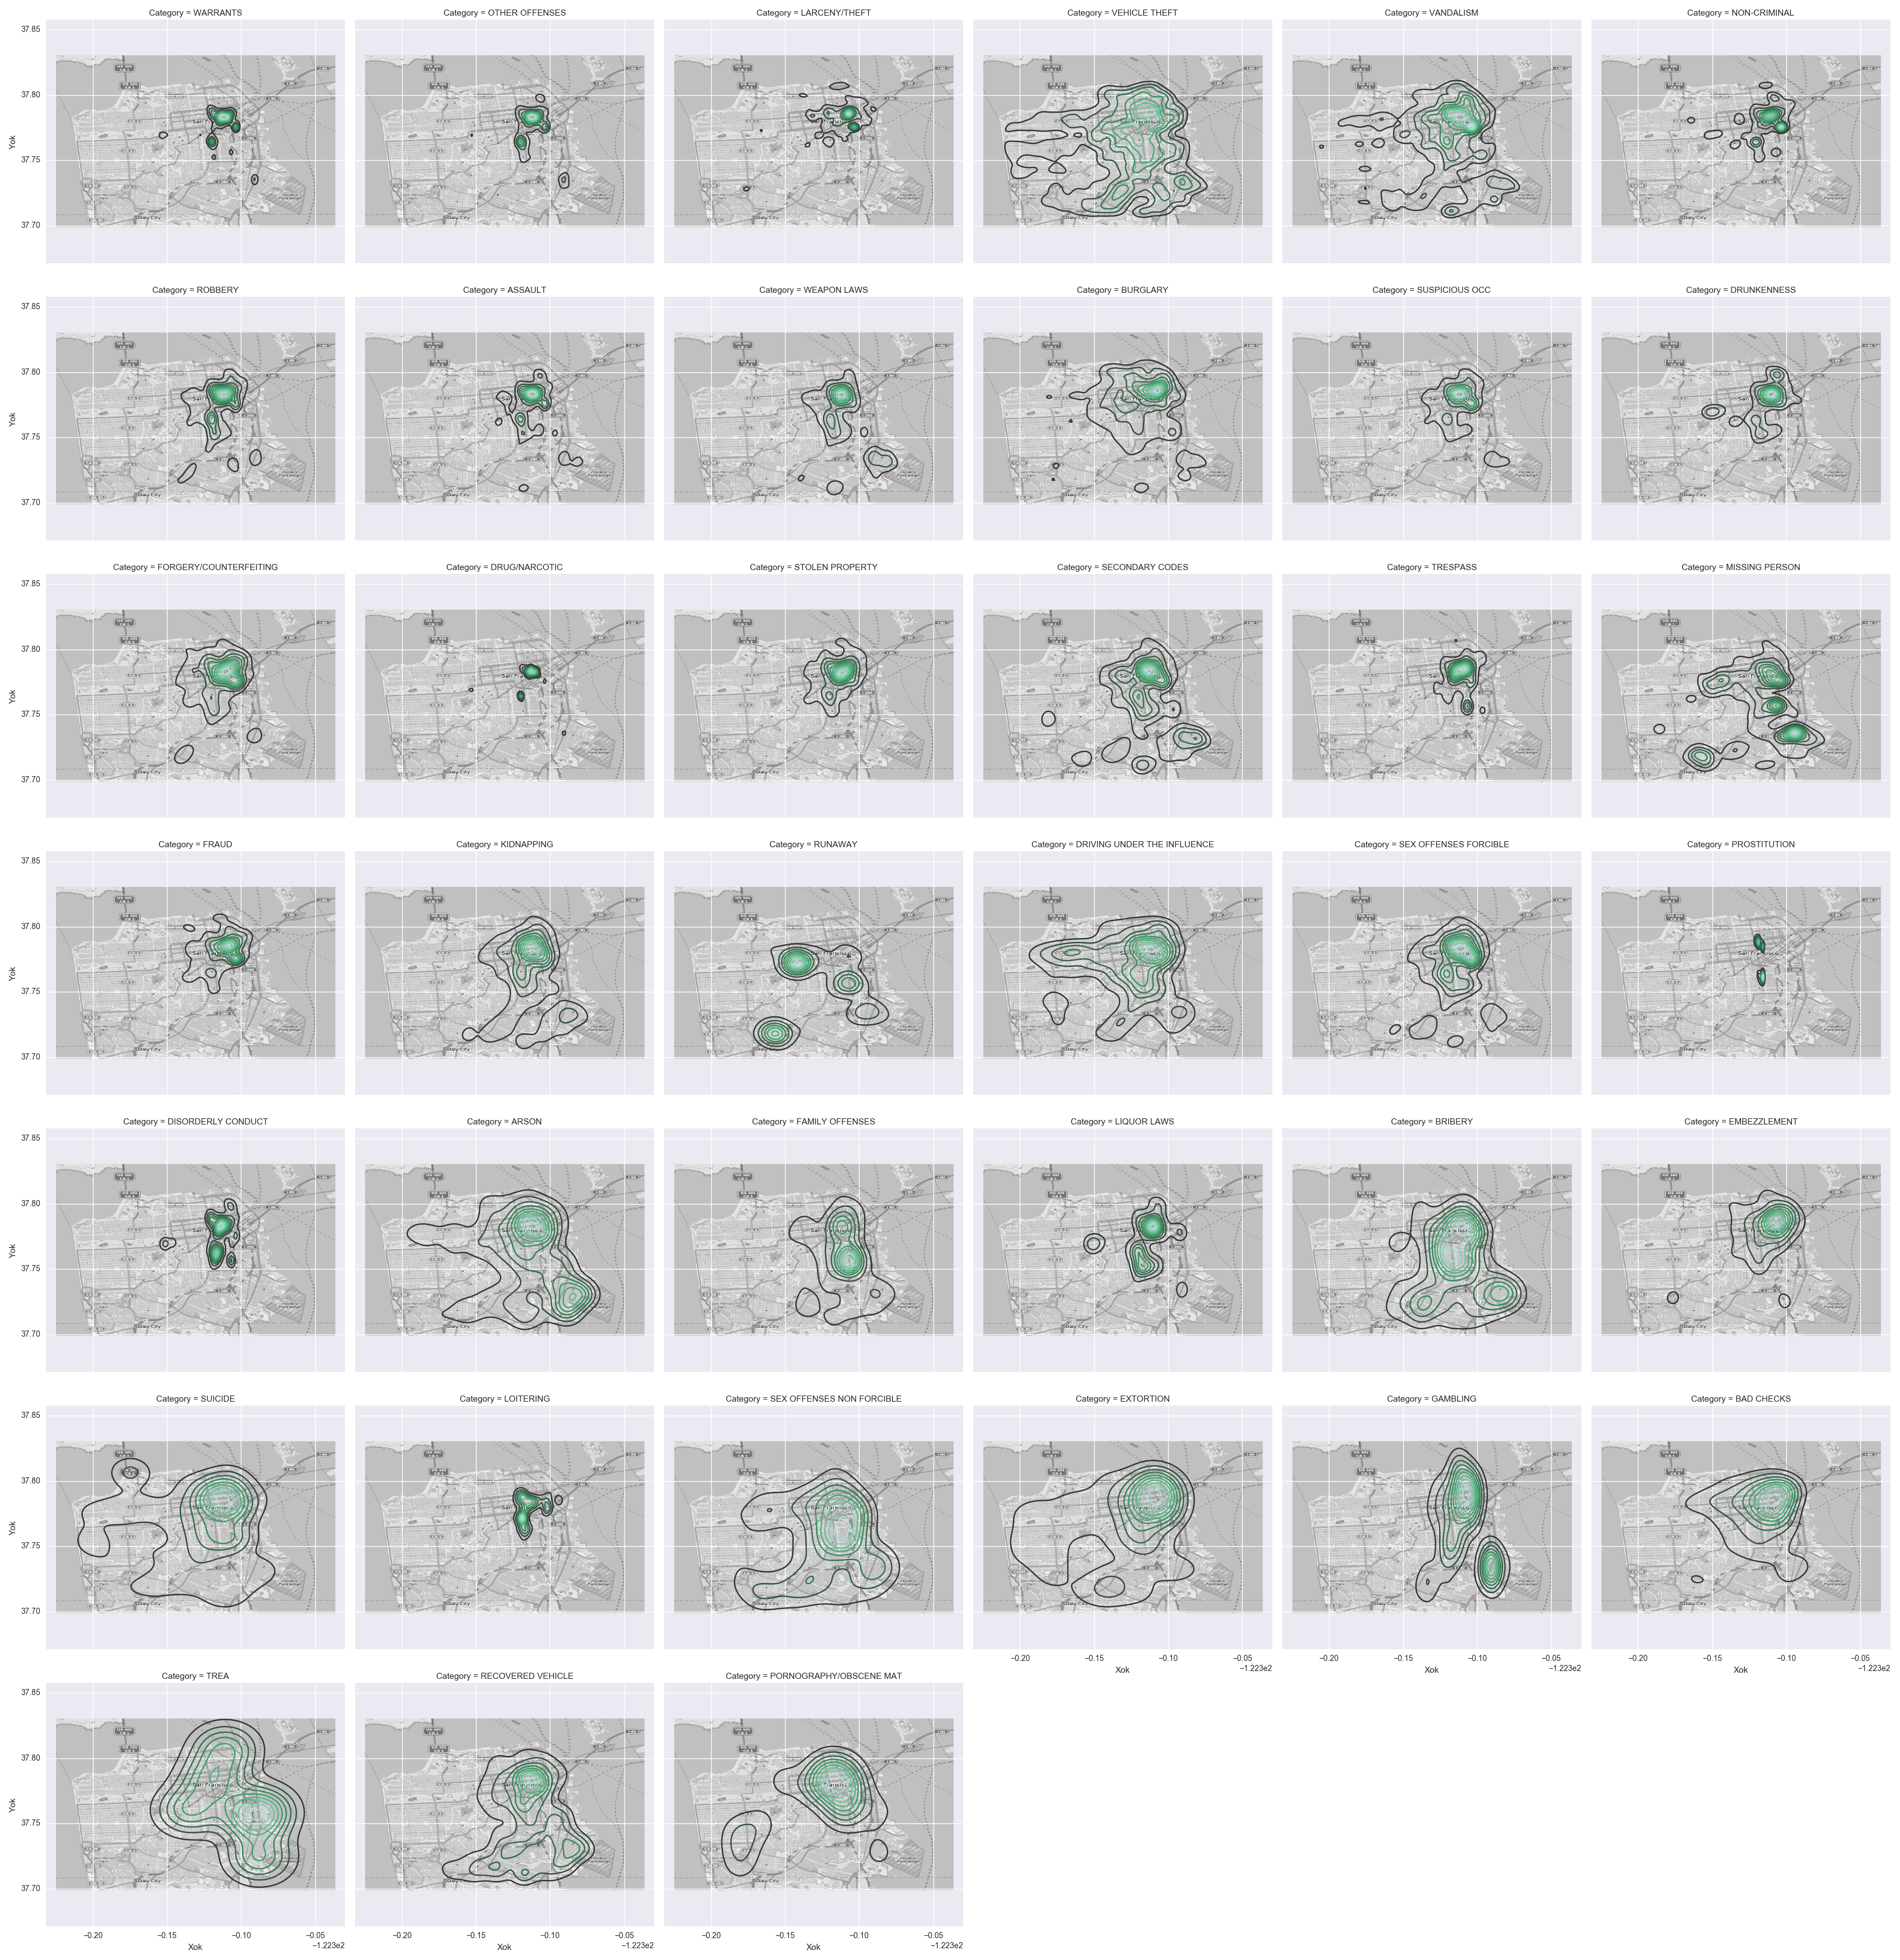
\includegraphics[width=1.0\linewidth]{fig/category_density}
    \caption{每种犯罪类型的密度图}
    \label{fig:tot_category}
\end{figure*}

\newpage

\subsubsection{不同犯罪类型对时间的分布}

对于时间分布的分析,我们采用的方法是比较不同时间特征下,犯罪分布的相似程度。对于离散分布的相似性比较,我们使用的方法是计算两个分布的相关系数:

\begin{equation*}
r_{xy}=\frac{\sum^n_{i=1}(x_i-\bar{x})(y_i-\bar{y})}{\sqrt{\sum^n_{i=1}(x_i-\bar{x})^2\sum^n_{i=1}(y_i-\bar{y})^2}}
\end{equation*}

其中,$x_1, x_2, \dot, x_{39}$表示一个时间特征下的犯罪类型分布(即每种犯罪类型发生的概率);$y_1, y_2, \dot, y_{39}$表示需要比较的另外一个分布。如果两个分布接近,即几乎满足$y_i=x_i$,则线性相关程度较高,计算出的相关系数也会越接近1。否则,如果分布差异很大,则计算出的结果会更接近0。可见,使用相关系数比较离散分布的相似性是合理的。

\begin{figure}[H]
    \centering
    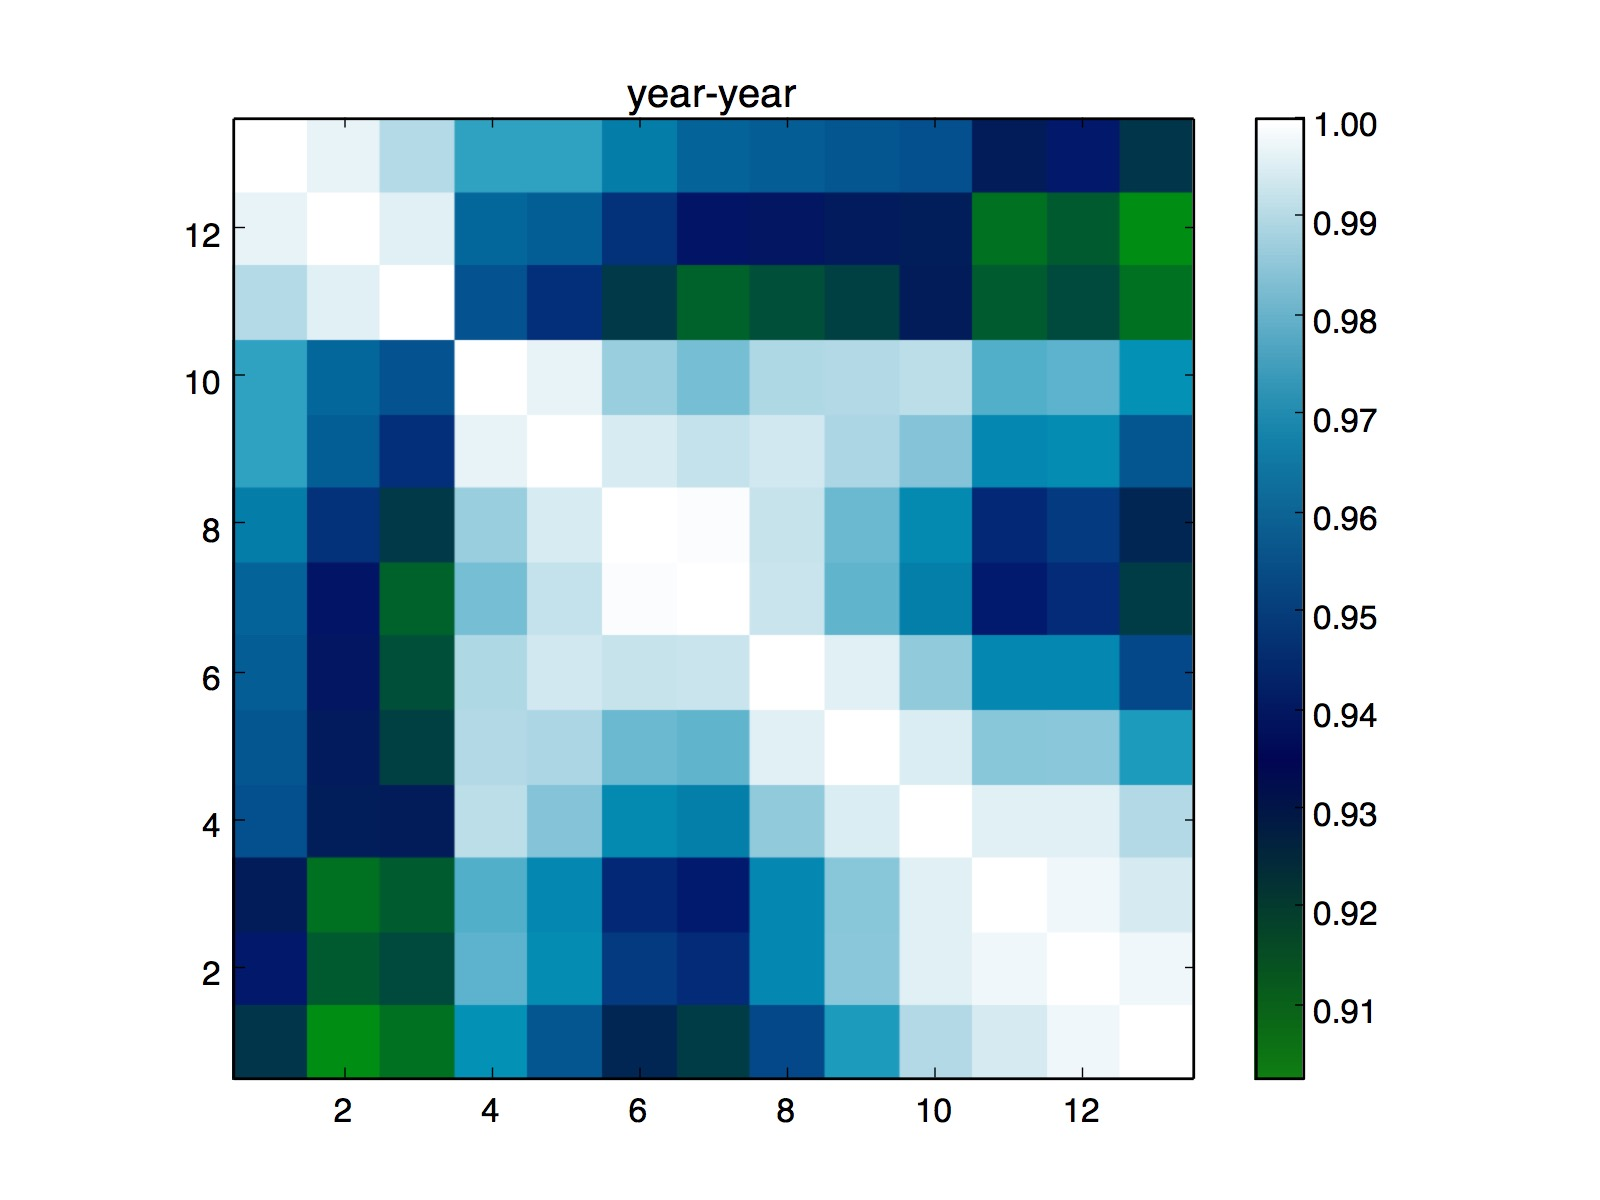
\includegraphics[width=1.0\linewidth]{fig/year_corr}
    \caption{不同年犯罪分布的比较}
    \label{fig:year_corr}
\end{figure}

从图\ref{fig:year_corr}可以看出,不同年份犯罪类型分布还是有一定差异的。特别地,我们看出一个明显的分界,那就是第3年(2005年)和第4年(2006年)之间。前三年的分布比较接近,后就九年的分布比较接近,而这两个时间段之间的差异还是比较大的。图\ref{fig:month_corr}中的结果则表明,不同月份之间的分布相似度都较大(相关系数最小的也有0.992),但是,也可以通过图中对角线的浅色区域看出月份越接近,犯罪分布越接近。图\ref{fig:weekday_corr}中则表明,每周各天的差异也比较小(相关系数至少有0.9855),但是也明显看出周末,即周五、周六、周日的犯罪分布十分接近,而一周中间的周三、周四和其他各天的犯罪分布的差异都比较大。

\begin{figure}[H]
    \centering
    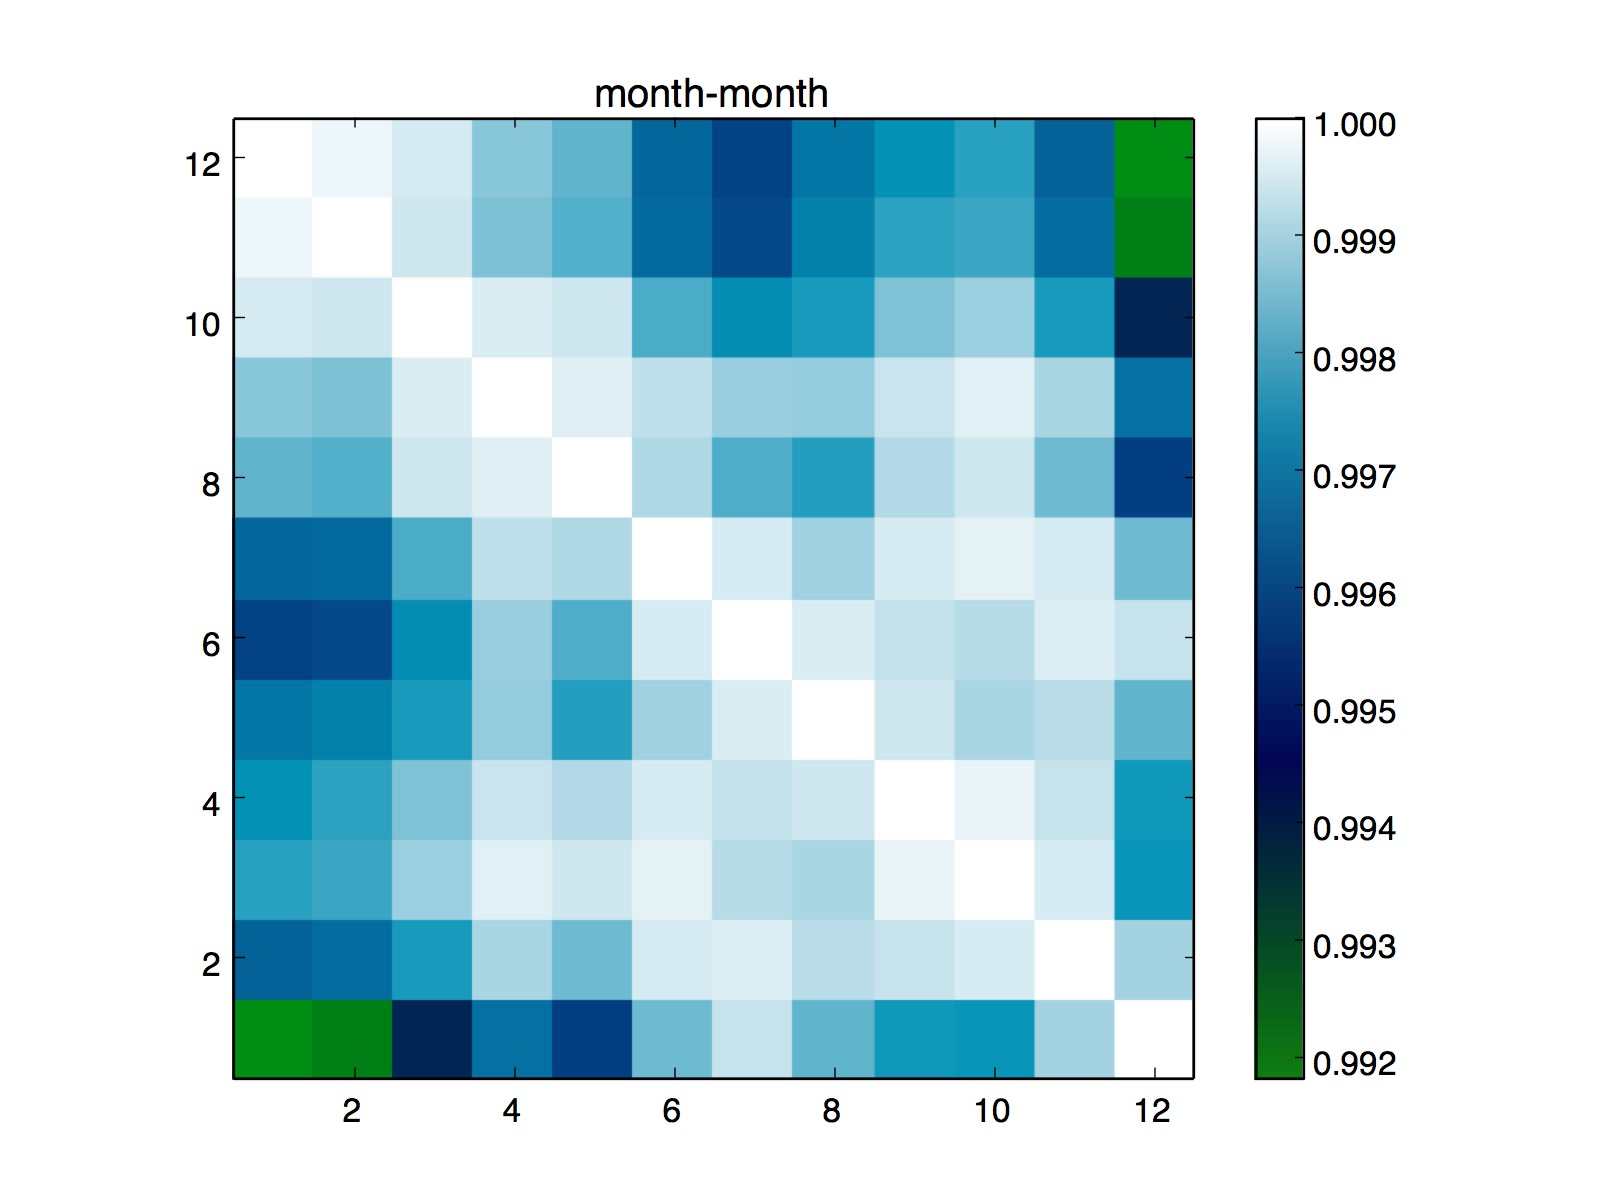
\includegraphics[width=1.0\linewidth]{fig/month_corr}
    \caption{不同月犯罪分布的比较}
    \label{fig:month_corr}
\end{figure}

\begin{figure}[H]
    \centering
    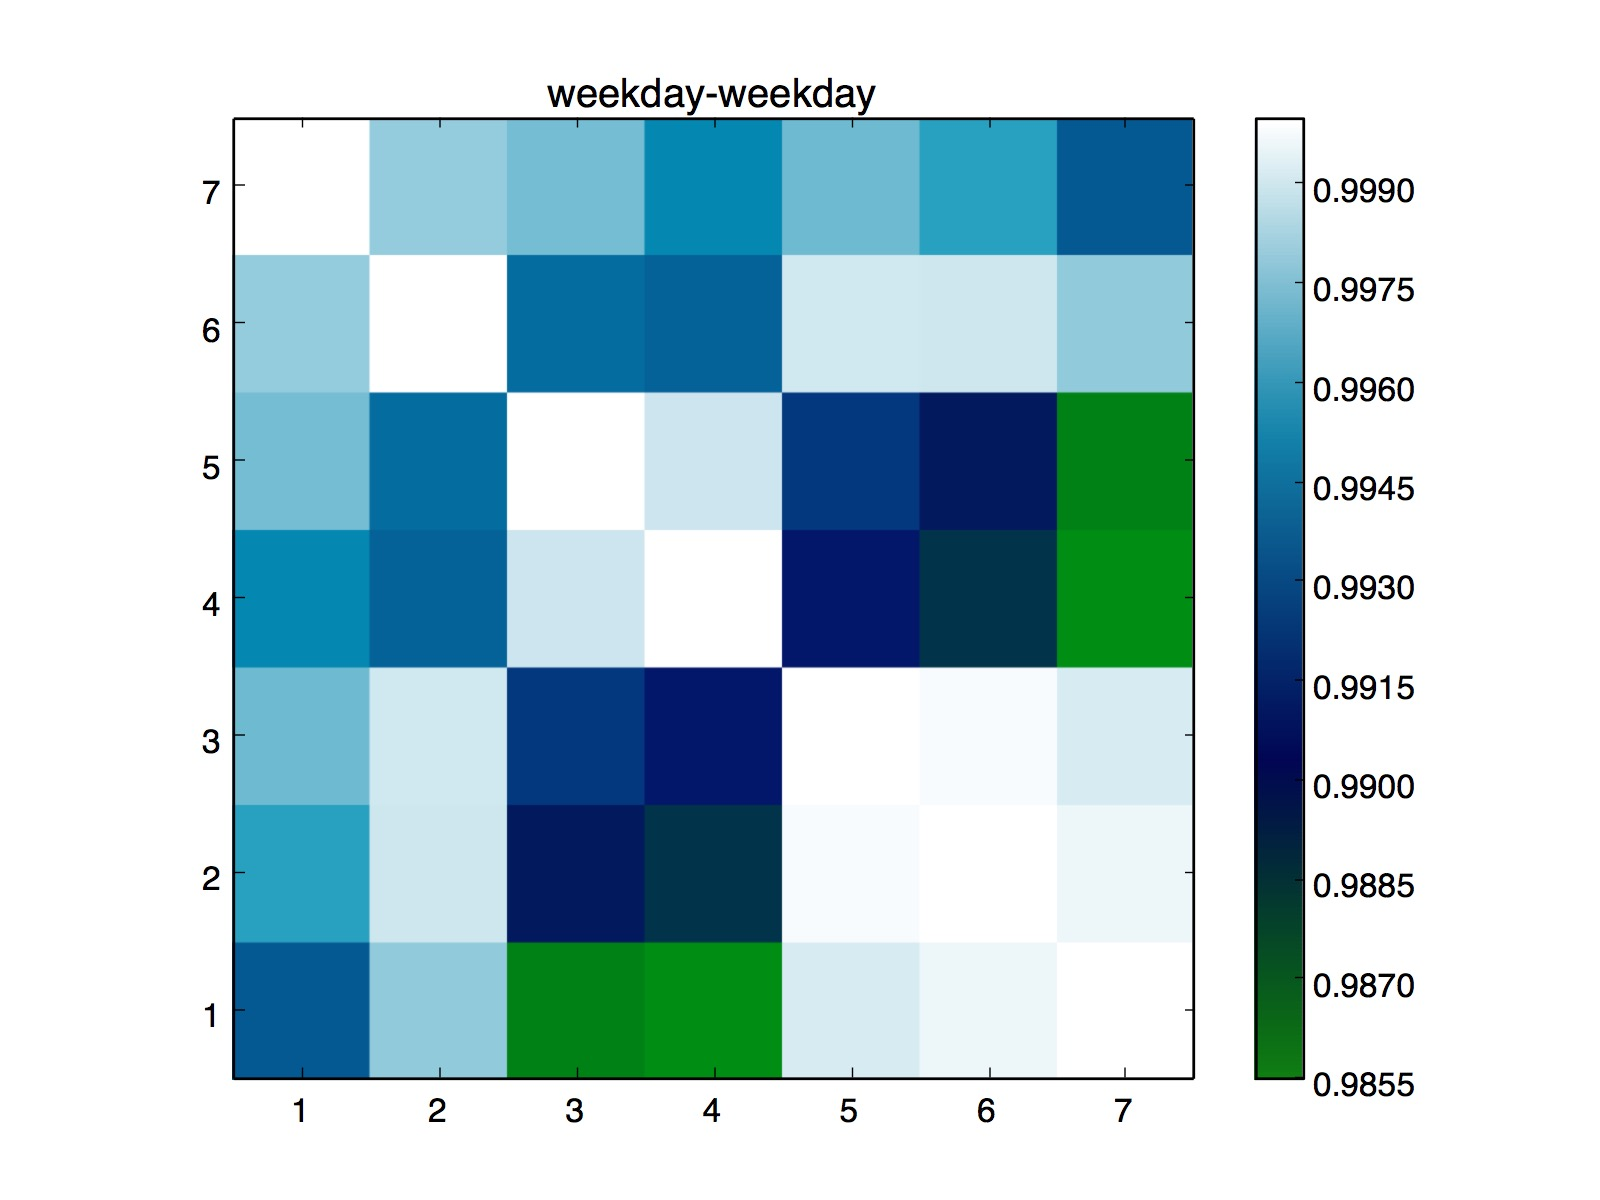
\includegraphics[width=1.0\linewidth]{fig/weekday_corr}
    \caption{每周各天的犯罪分布的比较}
    \label{fig:weekday_corr}
\end{figure}

\subsubsection{细粒度分析方法}

本部分对犯罪分布进行较细粒度的分析,即不仅仅考虑犯罪的总量,也要深入下去对每种不同的犯罪进行考虑。我们既关心不同犯罪类型在时间、空间上的分布是否不同,也关心不同的时间、地点下犯罪类型的分布(即一个$M=38$项的多项分布)是否不同。因此,我们不能仅仅考虑在全部时间段上的计数,而需要对考虑的时间做出一些限制。

\begin{figure}[H]
    \centering
    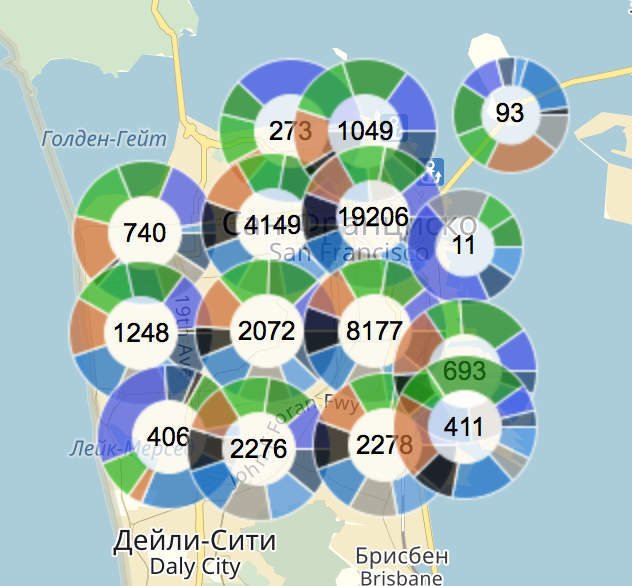
\includegraphics[width=1.0\linewidth]{fig/online_tool}
    \caption{在线分析工具给出的聚类结果}
    \label{fig:online_tool}
\end{figure}

这种细粒度的分析方式如果使用一个数据仓库是比较方便进行的,但数据仓库的实现十分复杂。在Kaggle论坛上,有参赛者公开了一个十分方便的交互式可视化分析工具\footnote{https://www.kaggle.com/tyz910/sf-crime/yet-another-map/notebook,作者Evgeny Ivanov。},可以起到数据仓库的作用。在这个工具中,我们可以对时间进行多种限制:指定日期区间、年份区间,指定某几个星期几和某几个小时。在此基础上,我们可以选定几个犯罪类别。该工具的输出是指定的犯罪类型,在指定的时间限制下,在地图上的聚类结果。同时,在每个聚类中心还会展示这个聚类中每类犯罪的分布情况。这个工具对于我们的探索分析是十分理想的。

图\ref{fig:online_tool}的结果便来自这个工具。图中给出了一定时间范围内,指定的几种犯罪的聚类结果和分布。可以再次验证不同地点的犯罪类型分布是不同的。同样,通过缩小时间范围,并比较不同时间范围的分布,也可以验证之前关于时间的发现,但其实不如我们之前的分析清晰,这里不再罗列。

经过数据可视化分析,我们可以明显地观察出地点和时间信息对于犯罪类型分布的影响。虽然我们发现的一些分布规律不容易直接应用到预测任务之中,但是,这种分析至少让我们可以肯定如果提取适当的特征、选择合适的模型,确实可以通过时间、地点信息推测出犯罪类型。




\section{特征工程}
\label{sec:feature}

\subsection{对原数据集进行数值化}
\label{subsec:feature0}

由于原始的数据集中的字段除了经纬度之外都是使用字符串形式给出的,为了方便后面的处理,我们先对各个字符串字段进行数值化。每个字段的数值化方法不只一种,除了直接对应为一个整数之外,也有更合理的方式进行数值化。

\textbf{Date} 对于时间戳字符串,我们直接把它进行分割,拆成6个字段,即年、月、日、时、分、秒。每个字段都是一个整数。每一个字段的大小关系都是有含义的(时间的先后顺序、接近程度),因此使用整数是比较合理的。除了直接对应外,也可以进行离散化,比如对一天中的时间进行分段。但是在实验中,我们并没有进行这种尝试。

\textbf{DayofWeek} 对于星期几这个字段,我们直接把星期一到星期天编码为整数1到7。这个字段使用整数编码是有意义的,整数的大小关系可以表示星期的先后。但是,由于星期是来回轮转的,因此使用一个7维二进制向量对星期进行编码也是合理的:比如,$[\begin{array}{ccccccc}1&0&0&0&0&0&0\end{array}]$表示星期一,$[\begin{array}{ccccccc}0&1&0&0&0&0&0\end{array}]$表示星期二。

\textbf{PdDistrict} 警察局字段一共有10个不同的取值。我们可以直接地映射到1到10十个整数,但是这种编码是不合理的,因为这会在警察局之间引入大小关系(线性关系),而这种关系实际是不存在的(即,人为加入了干扰信息)。所以,更合理的方式是,使用10维的二进制向量进行编码。

\textbf{Address} 地址信息的处理比较棘手。地址字段有三种形式:一个街道名;两个街道名;或者一个街道名和一个街区号。在训练集和测试集中,一共出现了2128种街道名称,我们首先按照字典序对街道进行整数编码(1到2128)。然后使用如下方式,用两个整数表示地址:

\begin{itemize}
    \item 两条街道名的地址:使用两街道的编号,小编号在前、大编号在后;
    \item 街道和街区号的地址:首先是街区号的相反数(小于等于0),然后是街道编号。
    \item 单一街道名:首先是街道编号,然后是-1。
\end{itemize}

这是从字符地址到整数的一种直接翻译,这些整数之间的大小关系、线性关系都是没有实际意义的。显然这不是一种很好的编码方法。但是,由于Kaggle比赛要求不能引入外界信息,我们无法使用街道的朝向和相互之间的位置关系对街道进行编码,只能使用字典序这种办法进行编码。
在实验中,我们只利用了地址中的街道信息。

至此,我们得到了数据集直接数值化后的特征。经过这一处理的特征,虽然数值化的方法仍有不合理之处,但我们已经可以用这个特征来训练模型了。

\subsection{对于街道进行犯罪概率统计}
\label{subsec:feature3}

由于我们对于街道的编码方式不合理,我们希望构造新的特征来更好地刻画街道的特性。一个直观的想法是,统计各个街道上的犯罪概率分布。首先,统计各个街道上39种犯罪的总数。对于每一个地址,使用如下步骤构造特征:

\begin{enumerate}
    \item 如果地址中出现了两条街道,则对两个街道的犯罪计数求和。否则就直接取所在街道的犯罪频数。
    \item 进行Laplace平滑处理,即对每一类的频数加1。
    \item 计算每种犯罪类型在该街道上的频率$p_j = \frac{f_j} {\sum_{k=1}^M f_k}$,其中,$f_j$是类别$j$的频数,$M$为总类型数39。
    \item 把每个频率$p$替换成$logodds(p)=log\frac{p}{1-p}$。这一处理可以更好地刻画频率之间的大小差距。
\end{enumerate}

至此,我们使用39个浮点数刻画了犯罪地点所在街道的犯罪类型特征。注意到,上面对每类犯罪频率的计算是考虑了整个训练集的,即在时间上的粒度是很粗糙的。但是,如果每个街道上实际存在一个犯罪分布,那么在更长的时间段中计数应该能更准确地计算这个分布,所以这样对全局计数是合理的。

\subsection{利用时空数据点的K-最近邻信息}
\label{subsec:feature4}

利用经纬度坐标信息,我们可以计算两个数据点之间的距离,由此可以采用K-最近邻方法来进行预测。除了直接进行预测外,也可以根据K-最近邻的结果构造特征。此外,考虑到除了接近的地点可能有类似的犯罪类型分布之外,接近的时间也可能有类似的犯罪类型分布。根据第\ref{sec:observation}节中的结果,在时间的分布上,月份(直接与季节、节日相关)和小时(白天和半夜的犯罪情况差别很大)应该对于犯罪有很大的影响。于是,我们构造了四维数据点$(\begin{array}{cccc}X, & Y, & Month, & Hour\end{array})$进行K-最近邻分析。

注意到,通过欧式距离计算最近邻的时候,需要对各个维度进行标准化。特别是对于本数据集构造的这种四维数据点。其中,$X$的$25\%$分位数和$75\%$分位数的差只有$122.43 - 122.40 = 0.03$,同时$Y$的$25\%$分位数和$75\%$分位数的差也为$37.78 - 37.75 = 0.03$。而刻画时间的两个维度都是整数,差至少为$1$,远远大于经纬度之间的差。如果不做标准化处理,则时间的差别会掩盖掉经纬度的差别,这样进行最近邻分析就没有意义了。因此,对于4位数据点的每一个维度,使用下面的方法进行标准化:

\begin{equation*}
    X' = \frac{X - \bar{X}}{s}
\end{equation*}

其中,$\bar{X}$为该维坐标的平均值,$s$是该维全体坐标的标准差。由这些坐标点得到的K-最近邻信息,我们可以使用两种办法编成特征。其一,直接把KNN模型的预测概率结果作为特征;其二是根据最近邻的距离进行加权得到每个犯罪类型的权值。加权的方式,可以简单地对距离取倒数,即类型$i$的权重为:

\begin{equation*}
    w_i = \sum_{j=1}^N\frac{1}{d_{ij}}
\end{equation*}

\subsection{利用聚类结果构造特征}
\label{subsec:feature5}

对于一种犯罪,我们根据生活经验,认为其具有一定的空间局部性,就是说某些区域发生某种犯罪的几率会比较高。因此我们决定做一些处理来体现空间局部性。

对于每种犯罪,我们统计所有该种犯罪的记录的地点信息,可以得到二维平面点的信息,这些数据使用K-means算法进行聚类。但是对于一种犯罪,有几个犯罪中心实际上
是不确定的,K-means算法也不能自动分辨出有几种类别。为了解决这个问题,我们枚举了类别数进行计算,为了度量分几类最好,我们将数据分为两折,一折用来聚类,另
一折用来测试,用在测试集上和在训练集上的相对误差来选取一个最好的分类数。

如此,我们便得到了每种犯罪的若干中心,接下来我们把各个犯罪记录到每种犯罪的最近的中心距离计算出来,作为特征加入到特征向量之中。

\section{模型实验}
\label{sec:model}

\subsection{实验框架的实现}

\subsection{逻辑斯蒂回归}

\subsection{朴素贝叶斯}

\subsection{随机森林}

\subsection{Xgboost}
\section{结论}
\label{sec:conclusion}

本次Kaggle比赛,我们通过精心调试Xgboost模型,使用很基础的特征就取得了前4\%的成绩。同时,我们通过学习Kaggle论坛上的脚本,对数据进行了可视化处理和观察分析。我们在构造特征时从多个角度进行了尝试。实验的过程中,我们发现构造的特征对于预测只有负面效果。我们针对这一现象进行了进一步实验,并做出了两种解释:构造特征时引入了对于预测目标的提示导致在训练集上过拟合;选用的模型不能很好地利用特征中的信息。

通过本次参加Kaggle比赛的经历,我们学习到了很多数据挖掘的经验。在面对实际的数据挖掘问题的时候,首先要多尝试不同的模型,来得出哪些模型比较适合这个问题。另外,不能闭门造车地纯做特征工程,因为无效的特征不仅会降低最终模型
的准确率,而且会增加模型的训练时间,因此增加特征值之后需要用模型对其进行检测,摒弃其中无效的部分;也不能纯凭自己的想法添加特征,应当结合对数据的分析;还要考虑当前使用的模型的表达能力是否足够利用这些特征。
另外,在模型调参的过程中,要去思考模型的特性,贴合实际问题去调整参数,如果训练速度较快,可以使用自动的调参工具(Grid Search)来进行参数的选择。
最后就是要相信测试集上交叉检验的结果,当出现提交结果与本地分折测试结果相差较大的时候,通常是自己在某些方面犯了错误,应当将其找出并修复。




%\bibitem{IEEEhowto:kopka}
%H.~Kopka and P.~W. Daly, \emph{A Guide to \LaTeX}, 3rd~ed.\hskip 1em plus
%  0.5em minus 0.4em\relax Harlow, England: Addison-Wesley, 1999.

%\end{thebibliography}

% that's all folks
\end{document}


